\documentclass[11pt,wide]{article}

\usepackage[T1]{fontenc}
\usepackage[utf8]{inputenc}
\usepackage{polski}
\usepackage{lmodern}
\usepackage{amsmath,amsthm}
\usepackage{algpseudocode}
\usepackage{pgfplots}
\usepackage{enumerate}
\newtheorem{thr}{Twierdzenie}
\newtheorem{lem}[thr]{Lemat}
\newtheorem*{dfn}{Definicja}
\usepackage{graphicx}
\graphicspath{ {img/} }
\usepackage[export]{adjustbox}
\title{Analiza numeryczna(M) - Pracownia 2 - Zadanie 6\\
}
\date{Grudzień 11, 2016}
\author{Wojciech Balik}


\begin{document}

\maketitle                
\thispagestyle{empty}     
\tableofcontents          
\section{Postacie wielomianów}
Problem interpolacji dla danych punktów $(x_k, y_k)$ $(k = 0,1,...,n)$ ma w przestrzeni $\Pi_n$(przestrzeni wielomianów stopnia co najwyżej n) dokładnie jedno rozwiązanie.Można jednak przedstawić ten wielomian na różne sposoby.Najprostszą do skonstruowania jest postać Lagrange'a:
\begin{equation}
W(x) = \displaystyle\sum_{k = 0}^{n} y_k\lambda_k(x),\indent\lambda_k(x)=\displaystyle\prod_{\substack{j=0\\j \neq k}}^n \frac{x-x_j}{x_k-x_j}
\end{equation}
Nie jest ona jednak używana do celów praktycznych ze względu na to że obliczenie wartości $W(x)$ ma złożoność obliczeniową $O(n^2)$ a duża liczba wykonywanych operacji arytmetycznych może stwarzać dość duże błędy numeryczne.Wadą tej postaci jest także to że dodanie nowego węzła interpolacyjnego zmusza nas do obliczania wszystkich współczynników od nowa.
\newline
Zdefiniujmy:
\begin{equation}
\lambda(x) = (x-x_0)(x-x_1)\ldots(x-x_n) = \displaystyle\prod_{j=0}^n x-x_j
\end{equation}
\begin{equation}
w_k = \frac{1}{\displaystyle\prod_{\substack{j=0\\j \neq k}}^n x_k-x_j}
\end{equation}
Zauważmy że we wzorze $(1)$, $\lambda_k$ możemy zapisać w następującej postaci:
\begin{equation}
\lambda_k(x) = \lambda(x) \frac{w_k}{x-x_k}
\end{equation}
Co po podstawieniu do wzoru (1) daje:
\begin{equation}
W(x) = \lambda\displaystyle\sum_{k=0}^n y_k\frac{w_k}{x-x_k}
\end{equation}
Załóżmy teraz że interpolujemy wielomian stopnia zerowego $Q(x) \equiv 1$ w punktach $x_0,x_1,\ldots,x_n$,wtedy:
\begin{equation}
Q(x) \equiv 1 = \lambda\displaystyle\sum_{k=0}^n \frac{w_k}{x-x_k}
\end{equation}
Dzieląc wzór (5) przez (6) otrzymujemy postać barycentryczną:
\begin{equation}
W(x)=\frac{\displaystyle\sum_{k=0}^n y_k\frac{w_k}{x-x_k}}{\displaystyle\sum_{k=0}^n \frac{w_k}{x-x_k}}
\end{equation}
Zauważmy że dla wartość $W(x)$ jest określona tylko dla $x \neq x_k$.Aby wielomian interpolacyjny był dobrze określony definiujemy:
\begin{center}
$P(x) = \begin{cases}
y_k & x = x_k , (k = 1,2,\ldots,n)\\
W(x) & wpp.\\
\end{cases}$
\end{center}
Wartości $w_k$ możemy obliczyć w czasie $O(n^2)$ ale gdy już to zrobimy, koszt obliczenia wartości wielomianu $P$ w punkcie $x$ to $O(n)$.Warto dodać że w przeciwieństwie do postaci Lagrange'a, dodając nowy węzeł interpolacyjny, możemy zaktualizować wartości $w_k$ w czasie liniowym.\newline

\noindent Ciekawą alternatywą jest  także postać Newtona:
\begin{equation}
W(x) = \displaystyle\sum_{k=0}^n a_k\displaystyle\prod_{j=0}^{k-1}x-x_j,\indent (\displaystyle\prod_{j=0}^{-1}\cdot \equiv 1)
\end{equation}
Dla ilorazu różnicowego zdefiniowanego jako:
\begin{equation}
f[x_0, x_1, \ldots, x_k] = \displaystyle\sum_{i=0}^k \frac{f(x_i)}{\displaystyle\prod_{\substack{j = 0\\j \neq i}}^k x_i - x_j}
\end{equation}
Współczynniki $a_k$ możemy zapisać w postaci:
\begin{equation}
a_k = f[x_0,x_1,\ldots,x_k]
\end{equation}
\noindent Zauważmy że używając wzoru rekurencyjnego:
\begin{equation}
f[x_i,x_{i+1},\ldots,x_{i+j}] = \frac{f[x_{i+1},\ldots,x_{i+j}] - f[x_i,\ldots,x_{i+j-1}]}{x_{i+j} - x_i}
\end{equation}
Możemy obliczyć współczynniki $a_k$ w czasie $O(n^2)$, gdzie w każdej iteracji wypełniana zostaje kolejna kolumna macierzy,korzystając z wyliczonych już wcześniej wartości:
\[
 \begin{matrix}
  f[x_0] &  &  \\
  f[x_1] & f[x_0,x_1] &  \\
  f[x_2] & f[x_1,x_2] & f[x_0,x_1,x_2] \\
  \vdots & \vdots & \vdots & \ddots\\
  f[x_n] & f[x_{n-1},x_n] & f[x_{n-2},x_{n-1},x_{n}] & \cdots & f[x_0,x_1,\ldots,x_n] \\
 \end{matrix}
\]
\noindent
Szczegóły można doczytać w \cite[s.312]{kincaid}

\section{Algorytmy związane z interpolacją wielomianową}
\subsection{Obliczanie wartości wielomianu interpolacyjnego}
Jak już zostało wspomniane, postać Lagrange'a jest dość niewygodna ze względów praktycznych.Lepszym pomysłem jest obliczenie wartości $w_i, (i = 0,1,\ldots,n)$ postaci barycentrycznej, podanych we wzorze (3).Możemy to zrobić za pomocą algorytmu:
\begin{enumerate}
\item $M_0^{(0)} := 1$
\item $M_k^{(0)} := 0,\quad (k = 1,2,\ldots,n)$
\item Dla każdego $i = 1,2,\ldots,n \quad k = 0,1,\ldots,i-1$ wykonaj: 
\begin{enumerate}
\item $M_k^{(i)} := M_k^{(i-1)}/(x_k - x_i)$
\item $M_i^{(k+1)} := M_i^{(k)} - M_k^{(i)}$
\end{enumerate}
\item $w_i := M_i^{(n)}, \quad (i = 0,1,\ldots,n)$
\end{enumerate}
\noindent
Okazuje się że jeśli punkty $x_0,x_1,\ldots,s_n$ uporządkujemy względem średniej $\overline{X} = \displaystyle\sum_{k=0}^n x_k/(n+1)$, czyli:

\begin{equation}
x_i \prec x_j \Leftrightarrow |x_i - \overline{X}| < |x_j - \overline{X}|
\end{equation}
\noindent
To wpływa to pozytywnie na otrzymany wyniki, pod względem potencjalnych błedów numerycznych powastałych w wyniki wykonania algorytmu.(O inncyh sposobach porządkowania punktów $x_k$ można doczytać w \cite{werner})

\subsection{Zamiana postaci Lagrange'a na postać Newtona}
Załóżmy że mamy dane współczynniki $\sigma_k$ wielomianu w postaci Lagrange'a(1):
\begin{center}
$W(x) = \displaystyle\sum_{k = 0}^{n} \sigma_k\displaystyle\prod_{\substack{j=0\\j \neq k}}^n x-x_j$
\end{center}
\begin{center}
$\sigma_k = \frac{f(x_k)}{\displaystyle\prod_{\substack{j=0\\j \neq k}}^n x_k-x_j}$
\end{center}
Wtedy z definicji ilorazu różnicowego:
\begin{equation}
a_k = \displaystyle\sum_{i=0}^k \sigma_i \displaystyle\prod_{j = k+1}^n (x_i - x_j), \indent (k = 0,\ldots,n)
\end{equation}
Wówczas wartości $a_k$ można obliczać następującym algorytmem, operując na macierzy M rozmiaru $(n+1)\times (n+2)$:
\newpage

\begin{enumerate}
\item $M_i^{(0)} := \sigma_i, \quad (i = 0,1,\ldots,n)$
\item Dla każdego $k$ od $0$ do $n$:
\begin{enumerate}
	\item $M_{n-k}^{(k+1)} := \displaystyle\sum_{i=0}^{n-k} M_i^{(k)}$.
	\item $M_i^{(k+1)} := (x_i - x_{n-k})M_i^{(k)}, \quad (i = n-k-1,\ldots,0)$.
\end{enumerate}	
\item $a_i := M_i^{(n+1-i)}, \quad (i = 0,1,\ldots,n)$
\end{enumerate}
\[
 \begin{matrix}
  \sigma_0     & (x_0 - x_n)\sigma_0 & (x_0 - x_n)(x_0 - x_{n-1})\sigma_0 & \ldots & \displaystyle\prod_{j = 1}^n (x_0 - x_j) & \displaystyle\prod_{j = 1}^n (x_0 - x_j)  \\
  \sigma_1     & (x_1 - x_n)\sigma_1 & (x_1 - x_n)(x_1 - x_{n-1})\sigma_1 & \ldots & \displaystyle\sum_{i=0}^1 \displaystyle\prod_{j = 2}^n (x_1 - x_j)\sigma_i & 0 \\
  \sigma_2     & (x_2 - x_n)\sigma_2 & (x_2 - x_n)(x_2 - x_{n-1})\sigma_2 & \ldots & 0 & 0  \\
  \vdots       & \vdots              & \vdots & & \vdots & \vdots\\
  \sigma_{n-1} & (x_{n-1} - x_n)\sigma_{n-1}        & \displaystyle\sum_{i=0}^{n-1} (x_i - x_n)\sigma_i & \ddots & \vdots & \vdots\\
  \sigma_n     & \displaystyle\sum_{i=1}^n \sigma_i & 0 & \ldots & 0 & 0 \\
 \end{matrix}
\]
Zapominając o pierwszej kolumnie ,widzimy że wartościami $a_k$ są elementy na przekątnej macierzy $M$
\subsection{Wnioski}
Zauważmy że przy implementacji powyższych algorytmów nie musimy korzystać z tablicy dwuwymiarowej, co pozwala na użycie jedynie $O(n)$ pamięci.Ponadto, algorytm (2.1) wykonuje $n(n-1)$ odejmowań oraz $\frac{n(n-1)}{2}$ dzieleń, w przeciwieństwie do algorytmu naiwnego(obliczania tych wartośći korzystając wprost ze wzoru z definicji) w którym występuje $n^2$ odejmowań oraz dzieleń.Powinno to zmniejszyć nie tylko czas wykonania, ale także ilość błedów numerycznych powstałych w wyniku zaokrąglania obliczanych wartości.

\section{Testy Numeryczne}
Obliczenia zostały przprowadzone w następujący sposób:
\begin{enumerate}
\item Zostało wylosowane 100 wielomianów stopnia co najwyżej 6
\item Każdy z tych wielomianów został zinterpolowany w $n$ równoodległych punktach na przedziale $[-10,10]$, na 4 sposoby:
\begin{enumerate}
\item Postać Lagrange'a, gdzie wartości są obliczane wprost ze wzoru (1)
\item Postać Newtona(używając algorytmu ilorazów różnicowych), wartości są obliczane za pomocą uogólnionego schematu Hornera
\item Postać Barycentryczna, wyznaczona poprzez algorytm (2.1)
\item Postać Barycentryczna, wyznaczona poprzez algorytm (2.1) z porządkiem względem średniej
\item Poprzez postać Lagrange'a, zmienonej na postać Newtona za pomocą algorytmu (2.2)
\end{enumerate}
Zatem jak już zostało wspomniane, dla $n>6$ istnieje dokładnie jeden taki wielomian interpolacyjny.W praktyce jednak, te wielomiany różnią się ze względu na błędy numeryczne powstałe poprzez poprzez zaokrąglenia przy wyznaczaniu współczynników wielomianów (a)-(e).Chcemy sprawdzić jak bardzo wartości otrzymanych wielomianów różnią się od wartości rzeczywistych.W tym celu dla każdej z metod (a)-(e):
\item Dla każdego ze stu wielomianów na przedziale $[-100,100]$ obliczamy błąd względny dla $1000$ punktów, sumujemy wszystkie błędy i uśredniamy wynik, dzieląc przez $1000$.
\item Podobnie jak w punkcie poprzednim, sumujemy średni błąd dla każdego wielomianu i dzielimy przez $n$, uzyskując średni błąd względny dla danego $n$
\end{enumerate}
\noindent
Poniższa tabelka prezentuje wyniki wyżej opisanych obliczeń, wykonanych używając arytmetyki podwójnej precyzji(double)

\begin{center}
\begin{tabular}{|c|c|c|c|c|c|}
  \hline 
  n & (a) & (b) & (c) & (d) & (e) \\ \hline
  7 & 2.045e-14 & 7.134e-12 & 1.829e-10 & 1.500e-10 & 1.162e-11\\\hline
  10 & 1.565e-12 & 8.546e-12 & 4.620e-06 & 4.080e-06 & 2.445e-11\\\hline
  13 & 4.523e-09 & 2.941e-09 & 2.030e-02 & 2.261e-02 & 4.101e-09\\\hline
  16 & 4.276e-05 & 7.042e-06 & 5.922e-01 & 5.110e-01 & 2.260e-05\\\hline
  19 & 4.455e-01 & 1.119e-01 & 6.638e-01 & 7.050e-01 & 2.843e-01\\\hline
  22 & 7.614e+03 & 1.870e+03 & 7.919e-01 & 8.282e-01 & 3.240e+03\\\hline
  25 & 5.464e+07 & 7.745e+06 & 8.012e-01 & 8.129e-01 & 3.977e+07\\\hline
  
\end{tabular} 
\end{center}
\noindent
Na poniższych wykresach można zobaczyć jak dane metody sprawdziły sie w interpolacji funkcji $arctg(x)$ oraz $\frac{1}{1 + 25x^2}$ \newline
\noindent
\begin{center}
Wykres dla funkcji $arctg(x)$ z węzłami równo odległymi: \newline
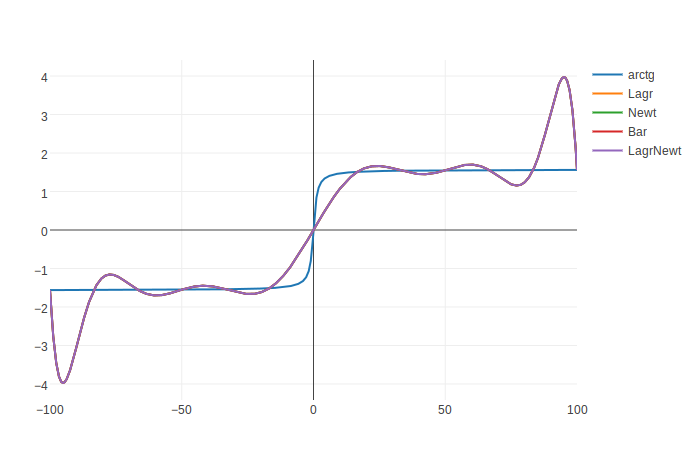
\includegraphics[scale = 0.55]{arctg}

Wykres dla funkcji $arctg(x)$ z węzłami Czebyszewa: \newline
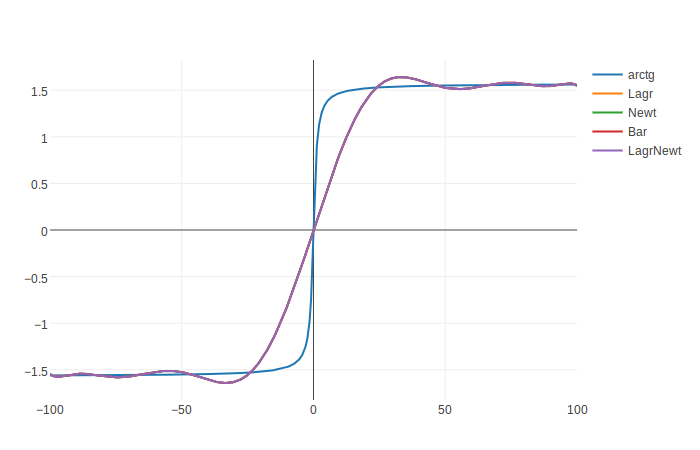
\includegraphics[scale = 0.55]{arctgch}

Wykres dla funkcji $\frac{1}{1 + 25x^2}$ z węzłami równo odległymi: \newline
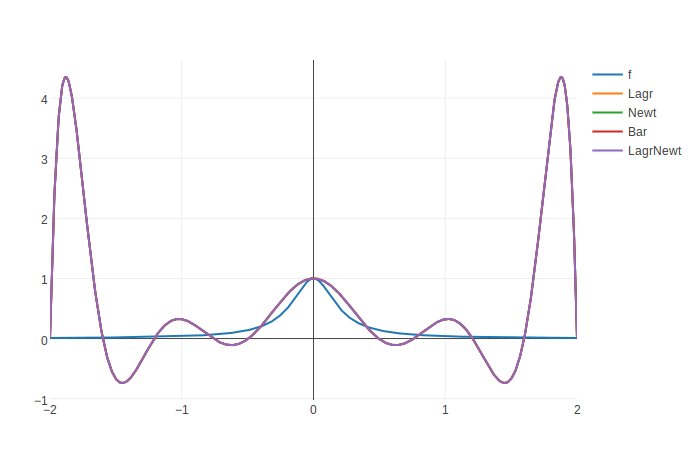
\includegraphics[scale = 0.55]{runge}

Wykres dla funkcji $\frac{1}{1 + 25x^2}$ z węzłami Czebyszewa: \newline
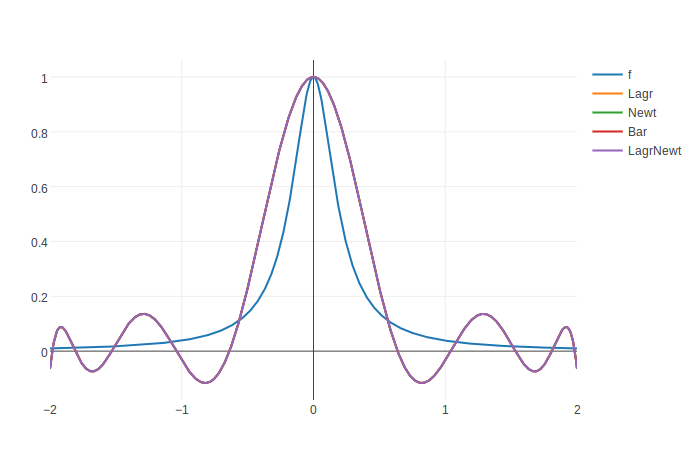
\includegraphics[scale = 0.55]{rungech}

\end{center}

\section{Podsumowanie}
Ze wszystkich postaci wielomianu interpolacyjnego, najlepszą okazała się postać Barycentryczna, ze względu na swoją stabilność numeryczną, łatwość w obliczaniu jej wartości oraz dodawania nowych węzłów interpolacyjnych.Algorytm wyznaczania jej współczynników co prawda generuje błędy numeryczne które można delikatnie zmniejszyć porządkując punkty $x_k$, lecz ogólnie rzecz biorąc, bilans zysków i strat jest dodatni.\newline\noindent
Algorytm przekształcania wielomianu z postaci Lagrange'a do postaci Newtona daje akceptowalne wyniki.Uzyskane współczynniki są nieco gorsze od tych obliczanych algorytmem ilorazów różnicowych, ale z kolei średni błąd względny jest mniejszy niż ten który otrzymujemy w przypadku obliczania wartości wielomianu w postaci Lagrange'a.\newline
Pozytywnym aspektem jest także to, że dla niewielkiej liczby węzłów interpolacyjnych, wielomiany otrzymane za pomocą powyższych metod nie różnią się prawie wcale, co widać na przedstawionych wykresach - różnica między wielomianami jest niezauważalna.

\begin{thebibliography}{10}
\bibitem{kincaid}
  David Kincaid, Ward Cheney,
  przekł. Stefan Paszkowski,
  \emph{Analiza Numeryczna},
  Warszawa, WNT, 2006.
  
\bibitem{werner}
 Wilhelm Werner,
 \emph{Mathematics of Computation 43 (1984) 205-217}
 
\bibitem{bertref}
 Jean-Paul Berrut
 Lloyd N. Trefethen
 \emph{Barycentric Lagrange Interpolation (2004)}
\end{thebibliography}


\end{document}